
\documentclass[a4paper, 12pt]{article}

\usepackage[utf8]{inputenc}
\usepackage[T1, T2A]{fontenc}
\usepackage[english, russian]{babel}
\usepackage{indentfirst}
\usepackage[top=2cm, bottom=2.5cm, left=2cm, right=2cm]{geometry}
\usepackage{graphicx}

\usepackage{pgfplots}
\pgfplotsset{compat=1.13}
\pgfplotsset{grid style={dashed, black}}

\usepackage{subcaption}

\usepackage{amsmath}

\usepackage{caption} 
\captionsetup[figure]{name = Рисунок, labelsep = endash}
\captionsetup[table]{name = Таблица, labelsep = endash, justification=raggedright, singlelinecheck=false}
\renewcommand{\baselinestretch}{1.5} 
\parindent=1.27cm
\usepackage{pdfpages}
\begin{document}
	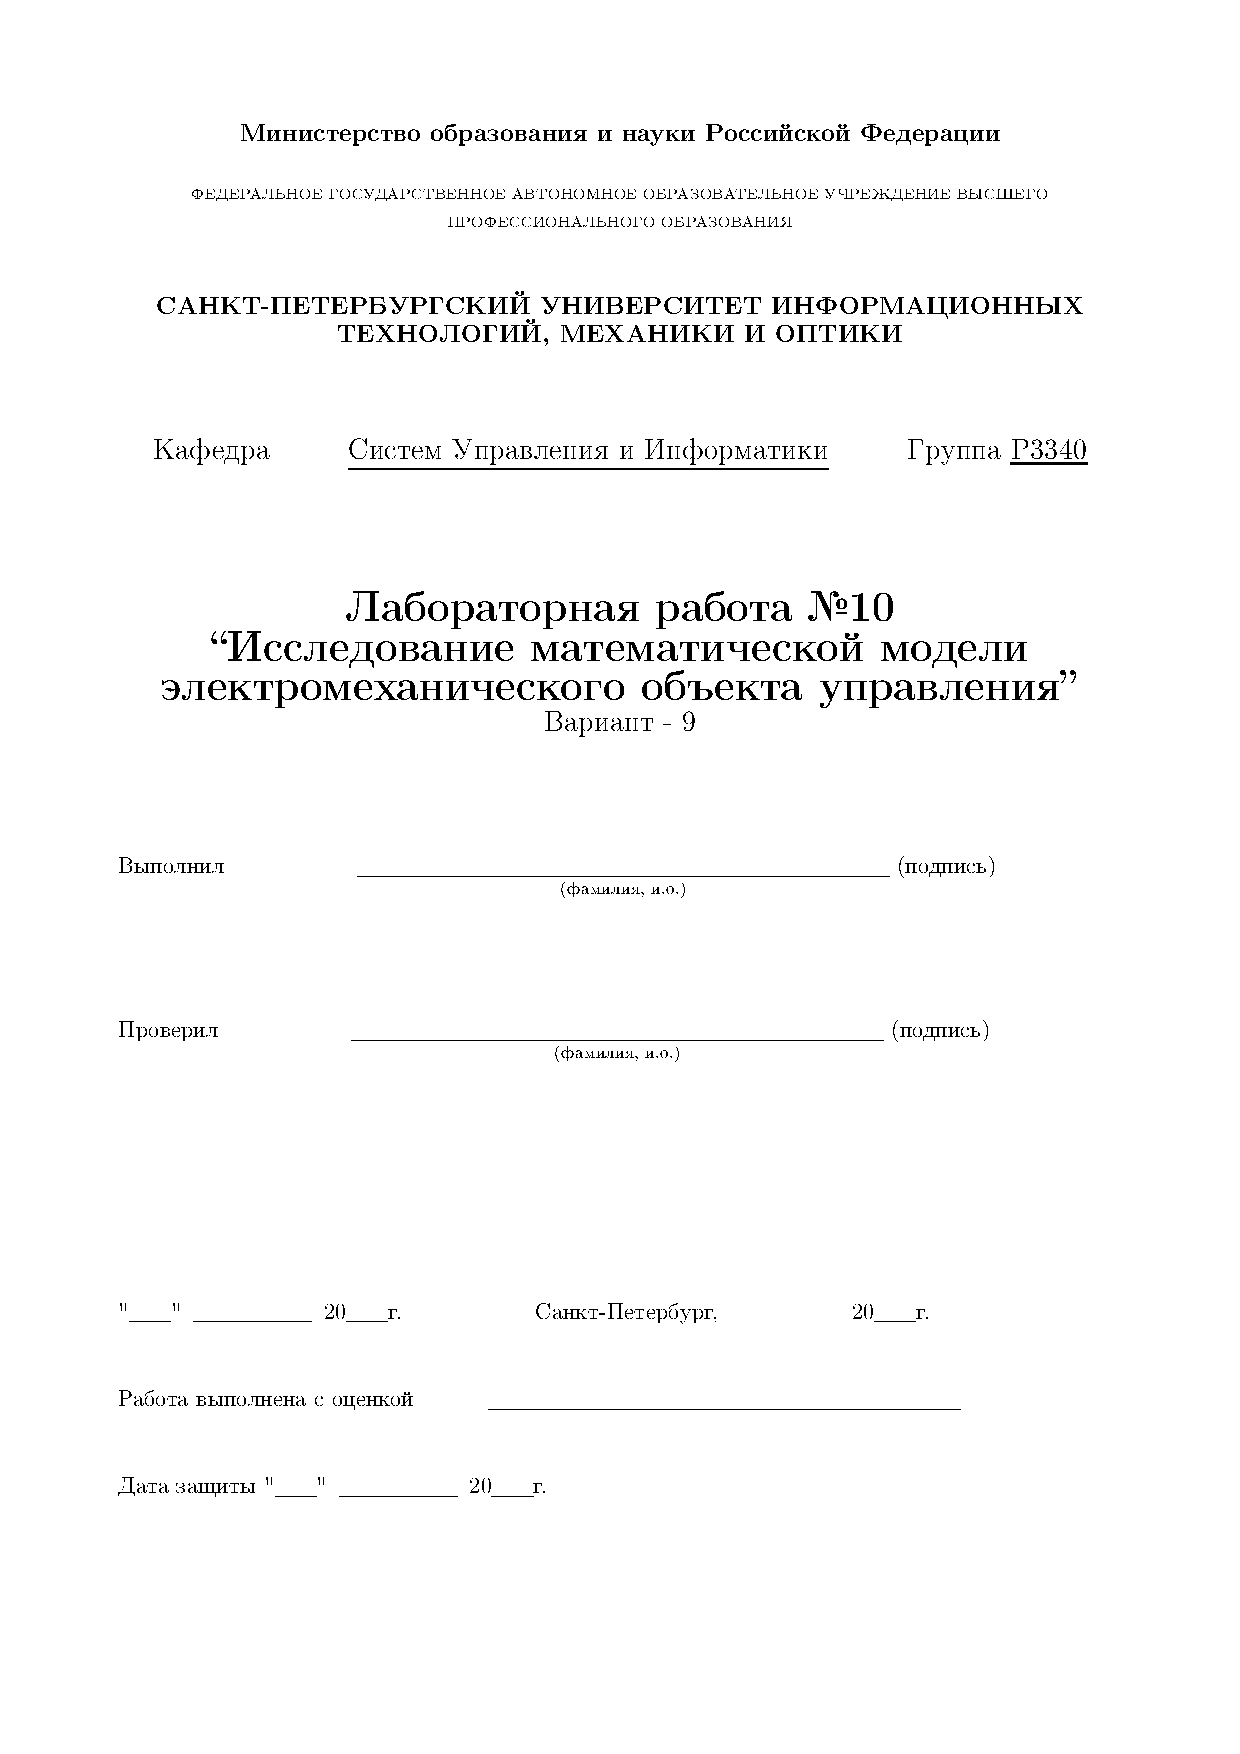
\includepdf{titul}
\paragraph{Цель работы:} Целью работы является изучение математических моделей и исследование характеристик исполнительного устройства, построенного на основе пьезоэлектрического двигателя микроперемещений\\
\paragraph{Начальные данные:}
	Структурная схема исполнительного устройства изображена на рисунке 1, параметры в таблице 1.
	\begin{table}[h!]
	\caption{Исходные данные}
	\renewcommand{\arraystretch}{1}
	\renewcommand{\tabcolsep}{0.7cm}
	\begin{tabular}{|c|c|c|c|c|c|c|}
		\hline
		Cp & m & K_0 & K_d & T_u & F_b & K_u\\
		
		Н/м&	кг&	Н/В&	Нс/м&	с&	Н&	Upm/Um\\
		\hline
		1.8*10^6&	0.01&	5.2&	0.7*10^2&	0.0002&	0.9&	30\\
		\hline
	\end{tabular}
\end{table}\par
\begin{figure}[h]
	\begin{center}
		\includegraphics[width=13cm]{struk}
		\caption{Структурная схема системы}
	\end{center}  
\end{figure}\par
Для соответствия выходного сигнала уровню 10, необходимо его домножить на коэффициент, рассчитанные коэффициенты:\\
Ku=0.033\\
Kf=0.033\\
Kv=2.73\\
Kx=11494 
\newpage
\begin{center}
\section{Исследование исполнительного устройства}
\end{center}\par
На рисунке 2 изображена схема моделирования устройства. На рисунке 3 - графики переходных процессов при нулевом внешнем воздействии.
\begin{figure}[h!]
\begin{center}
\includegraphics[width=11cm]{model}
\caption{Схема моделирования устройства}
\end{center}  
\end{figure}\par

\begin{figure}[h!]
\begin{minipage}[h]{0.49\linewidth}
\center{\includegraphics[width=1\linewidth]{Up} \\ Up}
\end{minipage}
\hfill
\begin{minipage}[h]{0.49\linewidth}
\center{\includegraphics[width=1\linewidth]{F} \\ F}
\end{minipage}
\vfill
\begin{minipage}[h]{0.49\linewidth}
\center{\includegraphics[width=1\linewidth]{V} \\ V}
\end{minipage}
\hfill
\begin{minipage}[h]{0.49\linewidth}
\center{\includegraphics[width=1\linewidth]{x} \\ x}
\end{minipage}
\caption{Графики переходных процессов при Fb=0 Н, U=10 В}
\end{figure}
\newpage
\begin{center}
\section{Исследование влияния массы нагрузки m на вид переходных процессов}
\end{center}\par
В таблице 2 приведена зависимость характеристик системы от массы нагрузки.
\begin{table}[h!]
	\caption{Характеристики системы при различной массе нагрузки }
	\renewcommand{\arraystretch}{1}
	\renewcommand{\tabcolsep}{0.9cm}
	\begin{tabular}{|c|c|c|c|c|c|c|}
		\hline
		m, кг	&	0.005	&	0.0075	&	0.01	&	0.0125	&	0.015	\\
		\hline
		tп,мс	&	1.2	&	1.2	&	1.25	&	1.5	&	1.7	\\
		\hline
		\sigma, \%	&	0	&	0	&	1	&	2	&	3	\\
		\hline
		x,10^{-3}м	&	0.87	&	0.87	&	0.87	&	0.87	&	0.87	\\
		\hline
	\end{tabular}
\end{table}
\newpage
\begin{figure}[h!]
\begin{minipage}[h]{0.49\linewidth}
\center{\includegraphics[width=1\linewidth]{m1} \\ m=0.005кг}
\end{minipage}
\hfill
\begin{minipage}[h]{0.49\linewidth}
\center{\includegraphics[width=1\linewidth]{m2} \\ m=0.0075кг}
\end{minipage}
\vfill
\begin{minipage}[h]{0.49\linewidth}
\center{\includegraphics[width=1\linewidth]{m3} \\ m=0.01кг}
\end{minipage}
\hfill
\begin{minipage}[h]{0.49\linewidth}
\center{\includegraphics[width=1\linewidth]{m4} \\ m=0.0125кг}
\end{minipage}
\begin{minipage}[h]{0.49\linewidth}
\center{\includegraphics[width=1\linewidth]{m5} \\ m=0.015кг}
\end{minipage}
\caption{Графики переходных процессов при изменении массы}
\end{figure}
\newpage
\begin{center}
	\section{Исследование влияния постоянной времени на вид переходных процессов}
\end{center}
Передаточная функция системы:\\
\begin{equation}
W(s)=\frac{K_UK_0}{T_Ums^3+(m+K_dT_U)s^2+(K_d+C_pT_U)s+C_p}
\end{equation}\par
В таблице 3 приведена зависимость характеристик системы от постоянной времени и расчитанные корни передаточной функции(1).   
\begin{table}[h!]
	\caption{Характеристики системы при различной массе нагрузки }
	\renewcommand{\arraystretch}{1}
	\renewcommand{\tabcolsep}{0.75cm}
	\begin{tabular}{|c|c|c|c|c|}
		\hline
		Tu,мс	&	0.2	&	0.4	&	0.8	&	1.2	\\
		\hline
		tп,мс	&	1.25	&	2	&	4	&	7.6	\\
		\hline
		\sigma, \%	&	0	&	0	&	0	&	0	\\
		\hline
		x,10^{-3} \text{ м}	&	0.87	&	0.87	&	0.87	&	0.87	\\
		\hline
		s_1, 10^{-3}	&	-5	&	-2,5	&	-1,25	&	-0,833	\\
		\hline
		s_2, 10^{-3}	&	-3.5-12.95i	&	-3.5-12.95i	&	-3.5-12.95i	&	-3.5-12.95i	\\
		\hline
		s_3, 10^{-3}	&	-3.5+12.95i	&	-3.5+12.95i	&	-3.5+12.95i	&	-3.5+12.95i	\\
		\hline
	\end{tabular}
\end{table}\par
На рисунке 5 приведены графики переходных процессов системы при изменении постоянной времени.
\newpage
\begin{figure}[h!]
\begin{minipage}[h]{0.49\linewidth}
\center{\includegraphics[width=1\linewidth]{t1} \\ Tu=0.2мс}
\end{minipage}
\hfill
\begin{minipage}[h]{0.49\linewidth}
\center{\includegraphics[width=1\linewidth]{t2} \\ Tu=0.4мс}
\end{minipage}
\vfill
\begin{minipage}[h]{0.49\linewidth}
\center{\includegraphics[width=1\linewidth]{t3} \\ Tu=0.8мс}
\end{minipage}
\hfill
\begin{minipage}[h]{0.49\linewidth}
\center{\includegraphics[width=1\linewidth]{t4} \\ Tu=1.2мс}
\end{minipage}
\caption{Графики переходных процессов при изменении Tu}
\end{figure}
\newpage
\begin{center}
	\section{Изучение вляния коэффициента упругости Cp на вид переходных процессов}
\end{center}\par
На рисунке 6, 7 приведены графики зависимости переходных процессов по положению и скорости от коэффициента упругости.
\begin{figure}[h!]
\begin{minipage}[h]{0.49\linewidth}
\center{\includegraphics[width=1\linewidth]{x12} \\ x при 0.5Cp}
\end{minipage}
\hfill
\begin{minipage}[h]{0.49\linewidth}
\center{\includegraphics[width=1\linewidth]{x22} \\ x при Cp}
\end{minipage}
\vfill
\begin{minipage}[h]{0.49\linewidth}
\center{\includegraphics[width=1\linewidth]{x32} \\ x при 2Cp}
\end{minipage}
\caption{Графики переходных процессов положения при изменении Cp}
\end{figure}
\newpage
\begin{figure}[h!]
\begin{minipage}[h]{0.49\linewidth}
	\center{\includegraphics[width=1\linewidth]{V21} \\ V при 0.5Cp}
\end{minipage}
\hfill
\begin{minipage}[h]{0.49\linewidth}
	\center{\includegraphics[width=1\linewidth]{V22} \\ V при Cp}
\end{minipage}
\vfill
\begin{minipage}[h]{0.49\linewidth}
	\center{\includegraphics[width=1\linewidth]{V23} \\ V при 2Cp}
\end{minipage}
\caption{Графики переходных процессов скорости при изменении Cp}
\end{figure}
\begin{figure}[h!]
	\begin{center}
		\includegraphics[width=14cm,height=6.8cm]{bode}
		\caption{ЛАЧХ системы}
	\end{center}  
\end{figure} 
\newpage
\begin{center}
	\section*{Вывод}
\end{center}\par
В лабораторной работе было исследованно пьезоэлектрическое исполнительное устройство. При исследовании влияния массы нагрузки на вид переходных процессов было выявлено, что при ее увеличении, увеличиваются колебания в системе и время переходного процесса.\par
При исследовании влияния постоянной времени, было выявленно, что при ее увеличении, увеличивается время переходного процесса, но при этом уменьшается перерегулирование.\par
Так же, при увеличении коэффициента упругости, увеличивается колебательность системы без изменения времени переходного процесса.
\end{document}